\documentclass[11pt, oneside]{article}
\usepackage[margin=1in]{geometry}
\geometry{letterpaper}
\usepackage{booktabs}
\usepackage{hyperref}
\usepackage{enumitem}
\usepackage{float}
\usepackage{caption}
\usepackage{subcaption}
\usepackage[numbers]{natbib}
\usepackage{graphicx}
\usepackage{amssymb}
\usepackage{amsmath}
\usepackage{array}
\usepackage{longtable}
\usepackage{xcolor}
\usepackage{tabularx}
\usepackage{setspace}
\usepackage{tikz}
\usetikzlibrary{arrows.meta,positioning,fit,calc}
\hypersetup{
    colorlinks=true,
    linkcolor=blue,
    citecolor=blue,
    urlcolor=blue,
    breaklinks=true
}
\newcommand{\githuburl}{https://github.com/AnshumaRaj/CS781-Capstone}
\graphicspath{{figures/}}

\title{CS781 Capstone Project:\\
In-House Legal Intelligence System}
\author{
    Anshuman Raj  \\
    240148 \\
    {\tt anshumanr24@iitk.ac.in}\\
    Indian Institute of Technology Kanpur (IIT Kanpur)\\[0.4em]
    {\small Public repository: \url{\githuburl}}
}
\date{}
\begin{document}
\maketitle
\begin{abstract}
Indian legal text is privileged, so I trained the stack on the official CS-781 corpus for on-premises use. I built one family of four from-scratch language models (50M--300M parameters, shared byte-level BPE, 1024-token block) and seven task heads on copies of those weights. My design question was how to reuse a compact decoder as a token encoder: rotary positions and grouped-query attention for pretraining, LoRMA and related PEFT for transfer, character-aligned windows for NER, sentence-level CRFs for roles, multi-window pooling for long judgments, and lexical first-stage retrieval where a 256-token neural view is too short. Official ranks and primary metrics are in Table~\ref{tab:leaderboard}; below I describe the architectures that produced them.
\end{abstract}

\section{Competition Result}
\noindent
\textbf{Codabench username:} a\_240148
\hfill
\textbf{Roll number:} 240148
\medskip

\noindent
Table~\ref{tab:leaderboard} is the system I selected for each phase, with rank as shown on the official board (freeze 9~November~2026). I uploaded at least four distinct systems per phase (four Phase-1 architectures, LoRMA, a second PEFT method, and a distilled encoder--decoder).

\begin{table}[H]
\centering
\small
\caption{Official selected system per phase. Rank is the live-board rank of that system on 9~Nov~2026.}
\label{tab:leaderboard}
\begin{tabular}{clccc}
\toprule
Phase & Task & Primary metric & Rank & Distinct zips \\
\midrule
1 & Legal LM pretraining & BERTScore F1 0.8328 & 55 & $\ge$4 \\
2 & Legal NER & strict macro-F1 0.5446 & 51 & $\ge$4 \\
3 & Rhetorical roles & macro-F1 0.5290 & 39 & $\ge$4 \\
4 & Court judgment prediction & macro-F1 0.6763 & 96 & $\ge$4 \\
5 & Statute identification & macro-F1 0.4252 & 23 & $\ge$4 \\
6 & Summarization & BERTScore F1 0.8503 & 22 & $\ge$4 \\
7 & Prior-case retrieval & Micro-F1@7 0.4519 & 33 & $\ge$4 \\
\bottomrule
\end{tabular}
\end{table}
\noindent
\textbf{Total valid Codabench submissions across all phases:} $\ge 35$.
\quad
\textbf{Date ranks were recorded:} 9~November~2026.

\section{Introduction and Problem Description}
A firm that holds Indian judgments cannot send them to a hosted API or initialise from a public legal BERT. I therefore built an in-house pipeline: one foundation family trained only on \texttt{Exploration-Lab/CS-781-Capstone}~\cite{cs781capstone}, then seven heads. Phase~1 continues a legal prompt for up to 128 words. Phase~2 extracts twelve entity types with exact character offsets. Phase~3 labels every provided sentence with one of thirteen rhetorical roles. Phase~4 predicts a binary outcome. Phase~5 assigns a subset of 100 masked statute IDs. Phase~6 writes a summary. Phase~7 returns seven prior cases from a split-specific pool.

The constraints that shaped my architecture were a 50M--300M parameter cap, no external corpora, a Tesla T4 memory budget, and strict span matching for NER. I did not train a single multi-task net and did not pipe Phase-2/3 outputs into later phases, because an offset error would propagate. I did not use public checkpoints or LLM APIs. Code is one starter-style notebook per phase at \url{\githuburl}.

\section{Data Analysis and Preprocessing}
\subsection{Sources and official splits}
All JSON comes from the official Hugging Face configuration. I counted Table~\ref{tab:splits} from the files I actually loaded.

\begin{table}[H]
\centering
\small
\caption{Official split sizes.}
\label{tab:splits}
\begin{tabular}{clccc}
\toprule
Phase & Unit & Train & Dev & Test \\
\midrule
1 & continuation prompts (test) & four official dumps & --- & 1000 \\
2 & documents (3 folds) & 35+35 & 8 held out of fold 2 & 35 \\
3 & documents (CL / IT) & 40 / 40 & 5 / 5 & 5 / 5 \\
4 & cases & 37\,387 & 1\,988 & 1\,517 \\
5 & documents, 100 labels & 42\,750 & 10\,181 & 13\,019 \\
6 & judgment / summary pairs & 7\,030 & --- & 100 \\
7 & queries / candidates & 827 / 4\,320 & 118 / 1\,023 & 237 / 1\,727 \\
\bottomrule
\end{tabular}
\end{table}

\subsection{Corpus statistics that informed design}
I pretrained on all four official dumps (Supreme Court, High Courts, Tribunals, and Central Acts), not on Supreme Court text alone. The hidden Phase~1 test is SC-style continuation, so I did not mix the four streams in equal volume. I drew about 50\% of tokens from the Supreme Court dump, 25\% from High Courts, 15\% from Tribunals, and 10\% from Acts. That split keeps the test register in the majority while still exposing the BPE and the model to High-Court citations, tribunal boilerplate, and statute wording. My byte-level BPE with a word-end marker keeps citation tokens (``AIR'', years, ``SCC'') as a few merges.

Phase~2 has twelve types. APP, RESP, COURT and STAT are common; WIT and R.COUNSEL are rare. Spans are short but can sit after several thousand characters of letterhead, so a word-limit that stops at 400 words never sees them. Adjacent APP/RESP mentions occur; nested spans are rare.

Phase~3 shares thirteen roles across corporate-law and IT. Fact, Argument and Ratio dominate; Dissent and PrecedentOverruled are almost absent, which is why I put a rare-role bias in the document-level CRF rather than adding a second encoder. I used the official sentence lists.

Phase~4 is binary. The operative sentence usually sits near the end of the judgment, so a head-only 512-token crop deletes the signal. Phase~5 has a long tail of statute IDs (about 3.7 labels per document) and the \emph{mentions} of those statutes are masked in the text. Phase~6 gold summaries overlap heavily with source $n$-grams and are much shorter than the judgments, which is why I chose sentence selection rather than free generation. Phase~7 queries and candidates are the same long, name-masked documents; I drop query IDs that also appear in the pool.

\subsection{Preprocessing}
I use the same BPE everywhere. I keep spaces and case so character offsets invert. Each BPE token stores \texttt{[start, end)} in the original UTF-8 string. For Phase~2 I slide overlapping 1024-token windows and merge duplicate spans. I do not re-segment Phase~3. For Phases~4--6 I pack a document as a few windows (head+tail or evenly spread). For Phase~7 I clip to 8\,000 words as two-thirds head plus one-third tail, matching how a reader skims a judgment.

\section{Approach and Model Evolution}
\subsection{Phase-1 foundation model}
My four architectures share a tied input/output embedding and a 1024-token block. None of them uses \texttt{nn.Transformer}. My \texttt{build\_model} refuses a count outside $[50,300]$ million.

\begin{table}[H]
\centering
\small
\caption{The four Phase-1 bodies. All share vocab 8192, block 1024, tied embeddings, and a \texttt{build\_model} check in $[50,300]$M.}
\label{tab:arch}
\begin{tabular}{lllc}
\toprule
Name & Attention / positions & MLP / norm & Params \\
\midrule
decoder & full causal MHA, learned pos. & GELU, LayerNorm & 110.2M \\
hybrid & 256-token window on 3/4 layers & same as decoder & 110.2M \\
efficient & RoPE, GQA 16Q/4KV & SwiGLU, RMSNorm & 118.5M \\
encdec & 6 bi-enc.\ + 6 causal+cross & GELU, LayerNorm & 106.3M \\
\bottomrule
\end{tabular}
\end{table}

My \textbf{decoder} is a pre-norm causal Transformer~\cite{vaswani2017attention}: width 1024, 8 layers, 16 heads. I used it as the control architecture---standard MHA with no rotary bias---so I can attribute later ablations to packing or PEFT rather than to a new positional scheme.

My \textbf{hybrid} keeps that size, but three of every four layers mask attention to a 256-token causal band. Local legal phrasing (``it is hereby ordered'', a statute short-title) then costs $O(n\cdot w)$ rather than $O(n^2)$. Every fourth layer is full causal attention so a citation at token 40 can still reach token 900. Residual connections and the FFN are unchanged, which is why the parameter count matches the decoder.

My \textbf{encoder--decoder} uses width 768, six bidirectional encoder blocks and six causal decoder blocks with cross-attention. I split a training block of 1024 tokens in the middle: the first half is the encoder source, the second half is teacher-forced on the decoder. I do \emph{not} use that split at task time; in Phase~6 I reuse the same weights with a full document as source and a summary as target.

My \textbf{efficient} model (width 1024, 10 layers) is the body I copied into most later phases. Rotary positions~\cite{su2024roformer} replace a learned table so relative distance is in the attention logits. RMSNorm replaces LayerNorm. The FFN is SwiGLU~\cite{shazeer2020glu} with an expansion that keeps the count near 118M. Grouped-query attention (16 query heads, 4 KV heads)~\cite{ainslie2023gqa} shrinks the KV cache on T4 without dropping to multi-query.

I trained a custom BPE~\cite{sennrich2016bpe} on a sample from all four dumps. A pair is merged only if it occurs at least twice; the score is Dice-weighted, $2C(xy)^2/(C(x)+C(y))$, so merges prefer cohesive legal pieces rather than fragments of ``the''. Bytes 0--255 are always in the vocab. I train with next-token cross-entropy, AdamW, block 1024, drawing blocks from the 50/25/15/10 mix above. I decode greedily and stop at EOS instead of padding to a fixed word count. In plain terms: the model always picks the most likely next token, and I cut the continuation when it emits the end marker, then keep at most 128 words.

\begin{figure}[H]
\centering
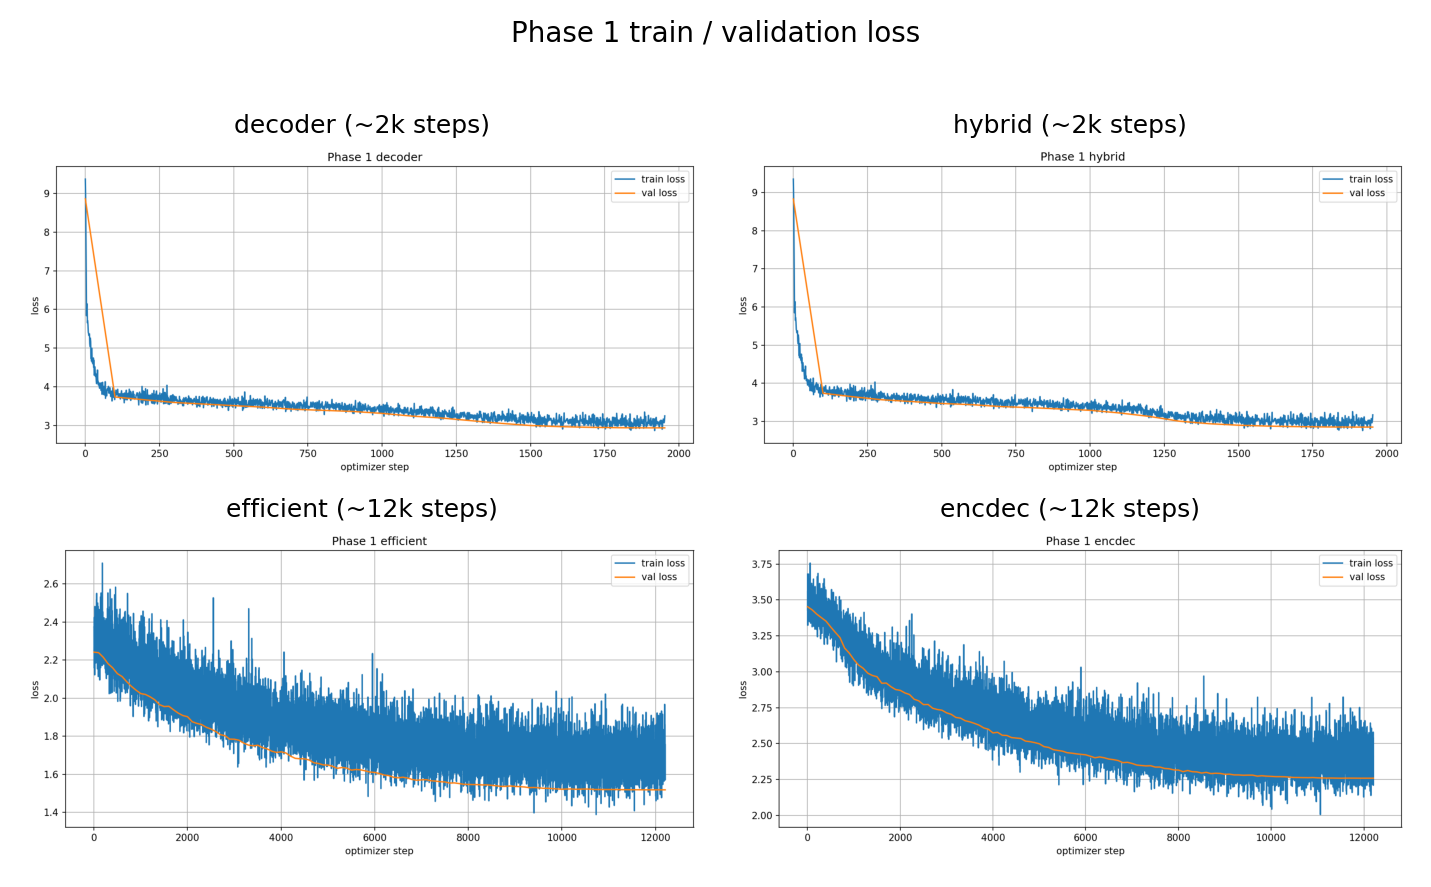
\includegraphics[width=0.98\linewidth]{p1_loss_grid.png}
\caption{Phase-1 train and validation loss. Decoder and hybrid were shorter runs ($\approx$2k steps); efficient and encoder--decoder ran longer ($\approx$12k). Validation tracks training on every body. I copied \emph{efficient} into most later heads and reused the encoder--decoder for extractive Phase~6.}
\label{fig:p1loss}
\end{figure}

\begin{figure}[H]
\centering
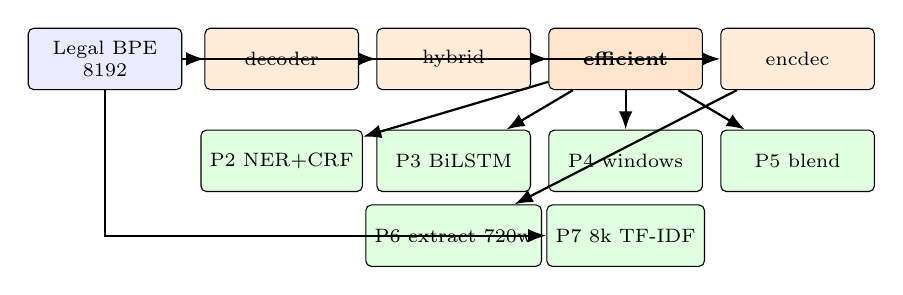
\begin{tikzpicture}[
  font=\scriptsize,
  box/.style={draw, rounded corners=2pt, align=center, inner sep=3.2pt, minimum width=1.95cm, minimum height=0.78cm},
  arr/.style={-{Latex}, thick}
]
\node[box, fill=blue!8] (tok) {Legal BPE\\8192};
\node[box, fill=orange!15, right=0.28cm of tok] (dec) {decoder};
\node[box, fill=orange!15, right=0.22cm of dec] (hyb) {hybrid};
\node[box, fill=orange!20, right=0.22cm of hyb] (eff) {\textbf{efficient}};
\node[box, fill=orange!15, right=0.22cm of eff] (enc) {encdec};
\node[box, fill=green!12, below=0.5cm of dec] (p2) {P2 NER+CRF};
\node[box, fill=green!12, below=0.5cm of hyb] (p3) {P3 BiLSTM};
\node[box, fill=green!12, below=0.5cm of eff] (p4) {P4 windows};
\node[box, fill=green!12, below=0.5cm of enc] (p5) {P5 blend};
\node[box, fill=green!12, below=1.45cm of hyb] (p6) {P6 extract 720w};
\node[box, fill=green!12, below=1.45cm of eff] (p7) {P7 8k TF-IDF};
\draw[arr] (tok) -- (dec);
\draw[arr] (tok) -- (hyb);
\draw[arr] (tok) -- (eff);
\draw[arr] (tok) -- (enc);
\draw[arr] (eff) -- (p2);
\draw[arr] (eff) -- (p3);
\draw[arr] (eff) -- (p4);
\draw[arr] (eff) -- (p5);
\draw[arr] (enc) -- (p6);
\draw[arr] (tok) |- (p7);
\end{tikzpicture}
\caption{Shared BPE and four Phase-1 bodies. Selected serving path: efficient for Phases~2--5, encoder--decoder extractive for Phase~6, lexical TF-IDF for Phase~7. The other bodies were PEFT and distillation vehicles, not a multi-task trunk.}
\label{fig:system}
\end{figure}

\subsection{Transfer protocol}
Every later phase loads a Phase-1 \texttt{state\_dict} and the same BPE. I adapt with LoRMA~\cite{bihany2025lorma}
\begin{equation}
h = \bigl(I + (\alpha/r)\,BA\bigr)Wx,
\end{equation}
with $B$ initialised at zero so the first step matches the frozen LM; LoRA~\cite{hu2022lora}; Houlsby adapters; partial unfreezing of the last $k$ blocks; BitFit; and response distillation from the efficient teacher into an encoder--decoder copy. I ran LoRMA on at least one architecture in every task phase. I used full fine-tuning of the efficient body only for NER, where the T4 still fits.

\subsection{Phase 2 --- Legal NER}
The scorer matches character intervals on the original string. So I never retokenise into words. I tag each BPE piece with a BIO label, then turn those tags back into \texttt{[start, end)} using offsets stored at encode time. A linear-chain CRF~\cite{lafferty2001crf} forbids illegal jumps such as \texttt{I-DATE} after \texttt{B-COURT}; Viterbi finds the best legal path. Judgments are longer than 1024 tokens, so I slide overlapping windows and keep the higher-scoring copy of a duplicate span. A light cleanup attaches APP to a neighbouring person-like mention and strips stray punctuation.

\textbf{Selected model.} Efficient body, \emph{full} fine-tune plus CRF, average of seeds 42 and 7. Full FT moved names that LoRMA left frozen. The required PEFT set I still submitted is efficient LoRMA, decoder full FT, hybrid LoRA, and encdec distillation; distillation failed when the distilled encoder--decoder did not inherit the offset tables.

\subsection{Phase 3 --- Rhetorical roles}
The unit is an official sentence, not a token. I mean-pool the Phase-1 hidden states of that sentence, so the LM is a sentence encoder. A BiLSTM then reads the whole judgment as a sequence of sentence vectors, and a CRF picks one of thirteen roles. Left/right context is therefore neighbouring sentences (Fact vs Argument), not extra subwords inside one sentence. Under LoRMA I freeze the sentence encoder; only the low-rank factors, the BiLSTM and the CRF train at full rate. Corporate-law and IT documents share the role set. I add a positive bias on Dissent and PrecedentOverruled in the CRF, because those labels are almost absent.

\textbf{Selected model.} Efficient LoRMA + BiLSTM-CRF + rarity bias. Other PEFT zips: decoder IA$^3$, hybrid LoRA, and an encoder--decoder copy distilled from the efficient LoRMA teacher.

\subsection{Phase 4 --- Court judgment prediction}
The holding is usually on the last page, so a 512-token head crop deletes the signal. I pack a case as several 256-token windows from head to tail, with extra mass on the ending. I mean-pool each window, a two-way linear head produces a logit, and I choose the decision cut on dev macro-F1 (accuracy is the wrong target on a two-class problem). I also encode the last $\approx$100 words as a bag-of-words ``ending cue'' and add it to the neural logit.

\textbf{Selected model.} Efficient body with only the last transformer blocks unfrozen (partial FT), plus the ending cue. That fits a batch of windows on a T4. I also submitted hybrid adapters, decoder BitFit, efficient LoRMA, and encoder--decoder distillation.

\subsection{Phase 5 --- Statute identification}
Mentions of the 100 statutes are stripped, so the model cannot copy a section number. I encode up to six 256-token windows of the efficient body. Each statute ID has its own query vector over tokens, plus a mean-pooled linear path whose bias is the label-frequency prior---not a shared 100-way softmax. Loss is binary cross-entropy. Empty predictions become the label with the largest score/threshold ratio. I fit a threshold \emph{per label} on a two-fold split of dev: a global cut of 0.5 cannot serve both frequent and rare IDs. Independently I train TF-IDF + per-label logistic regression on the same masked text (that is not a leak of section numbers).

\textbf{Selected model.} A blend of those neural logits with the TF-IDF model, then the per-label thresholds. Figure~\ref{fig:p5p6} shows why I serve the blend: PEFT-only heads sit well below it. The four-arch PEFT set I submitted is efficient LoRMA, decoder partial, hybrid adapters, and encdec distillation.

\subsection{Phase 6 --- Summarization}
I did train an abstractive path: causal models see document + BOS + summary with loss only on summary tokens; the encoder--decoder encodes the judgment and decodes the summary (I do \emph{not} reuse its Phase-1 half-block \texttt{forward}). That path is fluent but free to invent a holding. Gold summaries overlap the source, so I instead \emph{select} source sentences. I embed sentences with the encoder--decoder, score them by similarity to the document vector plus position (head/tail) plus lexical cues (\texttt{held}, \texttt{dismissed}), and greedily add a sentence if the 720-word budget still fits. A few head and tail sentences are forced so the holding is not dropped. Length control \emph{is} that budget.

\textbf{Selected model.} Encoder--decoder extractive ranker, 720 words. Figure~\ref{fig:p5p6} compares it with a 640-word extract and with abstractive LoRMA/KD on a local overlap proxy; official BERTScore is Table~\ref{tab:leaderboard}. I still ran LoRMA, partial FT, adapters and KD on the abstractive path to meet the PEFT requirement.

\begin{figure}[H]
\centering
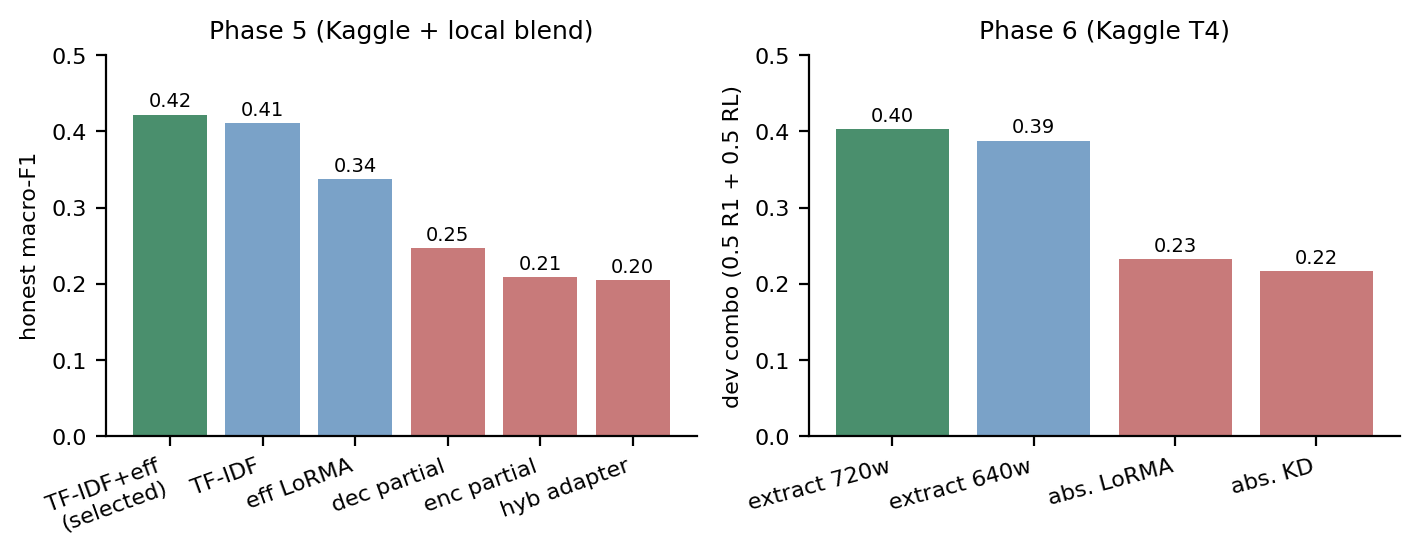
\includegraphics[width=0.98\linewidth]{p5p6_kaggle.png}
\caption{Architecture checks for Phases~5 and~6, not the official board. Left: local honest macro-F1 of the TF-IDF$\oplus$efficient blend versus PEFT-only heads. Right: local ROUGE-style overlap of extractive 720/640-word selectors versus abstractive LoRMA and KD. Official metrics remain Table~\ref{tab:leaderboard}.}
\label{fig:p5p6}
\end{figure}

\subsection{Phase 7 --- Prior-case retrieval}
Queries and candidates are long, name-masked judgments. I clip each document to 8\,000 words (two-thirds head, one-third tail), build a split-specific TF-IDF index (word $n$-grams 1--3, 400k features, sublinear TF), score cosine against the pool, drop the query's own ID, and return seven IDs. A citation-span field and a 1200-word head field are z-scored and added with small weights; they nudge the first stage, they do not replace it.

\textbf{Selected model.} That 8k TF-IDF + cite/head blend. Figure~\ref{fig:p7} is a development snapshot: stretching the clip to 12k or shrinking it to 3k does not beat 8k+fields, while a dual-encoder and a pair encoder that \emph{overwrite} the lexical list fall far behind. I still trained those neural jobs (InfoNCE on 4$\times$256 windows; a Phase-1 pair encoder on the TF-IDF top 20--30) to meet the PEFT/neural requirement, and kept them as ablations.

\begin{figure}[H]
\centering
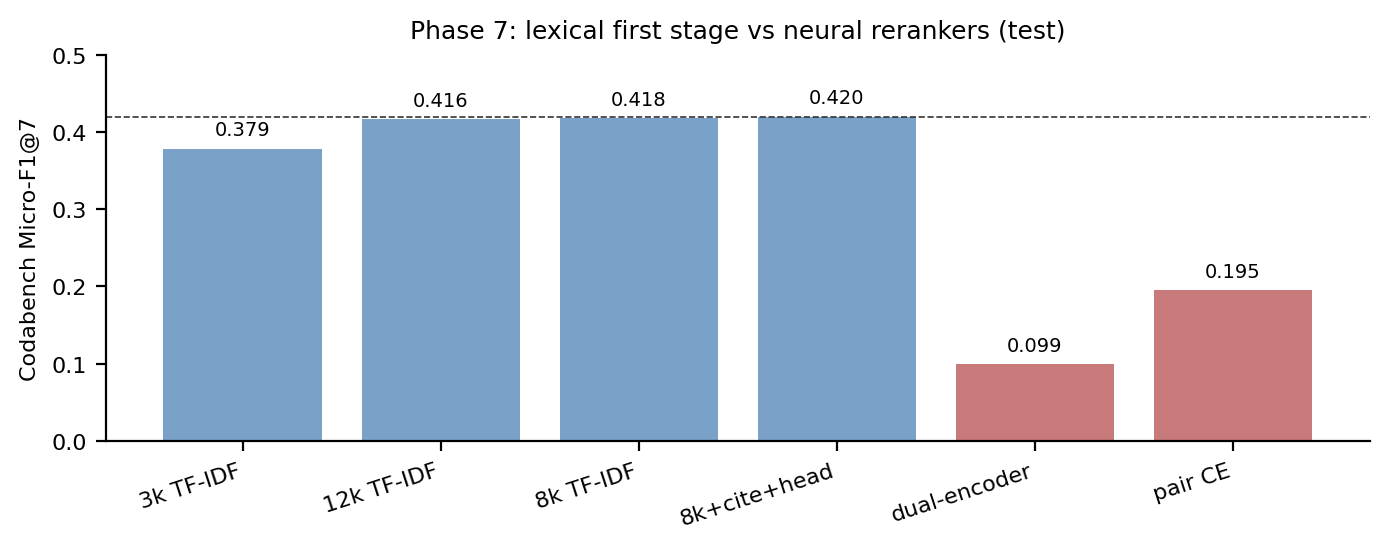
\includegraphics[width=0.82\linewidth]{p7_ablation.png}
\caption{Phase-7 architecture snapshot during development (not the official 0.4519 in Table~\ref{tab:leaderboard}). Lexical 8k + cite/head is the serving path; dual-encoder and pair-cross-encoder rerankers that replace the list do not.}
\label{fig:p7}
\end{figure}

\section{Experiments and Implementation Details}
\subsection{Compute and training protocol}
I ran neural jobs on Kaggle Tesla T4 (16\,GB, internet off, two concurrent kernels per account). Checkpoints write \texttt{best.pt} on the local metric; a \texttt{--train\_minutes} cap kills the job. I use AdamW (weight decay 0.01) and gradient clip 1.0. Dropout 0.1 sits only on newly added heads. I early-stop on span quality (P2), role macro-F1 (P3), thresholded macro-F1 (P4/P5), summary overlap (P6), and retrieval F1 on the 118 labelled queries (P7).

\begin{table}[H]
\centering
\scriptsize
\caption{Hyperparameters of the selected architecture in each phase.}
\label{tab:hparams}
\begin{tabular}{lccccccc}
\toprule
 & P1 & P2 & P3 & P4 & P5 & P6 & P7 \\
\midrule
Body & eff.\ GQA & eff.\ full & eff.\ LoRMA & eff.\ partial & blend & encdec rank & TF-IDF \\
Packing & 1024 blk & 1024 slide & sent pool & 6$\times$256 & 6$\times$256 & sentences & 8k words \\
Peak LR & $1\mathrm{e}{-4}$ & $2\mathrm{e}{-5}$ & $1\mathrm{e}{-4}$ & $2\mathrm{e}{-5}$ & $1\mathrm{e}{-4}$ & --- & --- \\
Batch & 8 & 2 & 1 doc & 4 & 2 & --- & --- \\
Schedule & $\approx$116M tok. & 5--8 ep. & 8 ep. & 6--8 ep. & 4 ep.+LR & extract & fit/split \\
Decode & greedy+EOS & Viterbi & Viterbi & dev $\tau$ & per-label $\tau$ & 720w & $K{=}7$ \\
\bottomrule
\end{tabular}
\end{table}

\subsection{Local evaluation}
I always hold out a subset of public train/dev. I run the official scripts under \texttt{evaluators/} before every upload (schema, unique IDs, offsets, exactly seven PCR IDs). Local and hidden test diverge when sklearn versions differ, when I use a ROUGE combo as a proxy for BERTScore, or when labelled dev is folded into training.

\subsection{Ablations}
I changed one factor at a time: Dice BPE versus count BPE; head+tail packing versus a cropped head; per-label versus global statute thresholds; extractive sentence rank versus abstractive continuation; TF-IDF first stage versus a dual-encoder or pair encoder on the same backbone; LoRMA versus full FT on NER. I kept the negative ablations in the code tree (pair rerank that overwrites the lexical list; 12k-word PCR that overfits 118 queries; a 400-word NER cutoff).

\section{Results}
Table~\ref{tab:leaderboard} is the official record. Table~\ref{tab:variants} names the architecture I selected and one runner-up. I used the efficient GQA decoder as the default neural body. Where the task is matching long, masked documents, I serve a linear or extractive system on the same corpus and keep the Phase-1 net as a PEFT/KD vehicle (Figure~\ref{fig:gap}).

\begin{table}[H]
\centering
\small
\caption{Selected architecture and a runner-up. Official numbers live in Table~\ref{tab:leaderboard}.}
\label{tab:variants}
\begin{tabular}{cll}
\toprule
Phase & Selected architecture & Runner-up \\
\midrule
1 & efficient, greedy+EOS & decoder / hybrid / encdec \\
2 & efficient full-FT + CRF, 2 seeds & efficient LoRMA+CRF \\
3 & efficient LoRMA + BiLSTM-CRF & hybrid LoRA / decoder IA$^3$ \\
4 & efficient partial + ending cue & efficient LoRMA \\
5 & TF-IDF $\oplus$ efficient windows & TF-IDF alone; PEFT-only heads \\
6 & encdec extractive, 720-word budget & abstractive LoRMA / KD \\
7 & 8k TF-IDF + cite/head fields & dual-encoder / pair-encoder \\
\bottomrule
\end{tabular}
\end{table}

\begin{figure}[H]
\centering
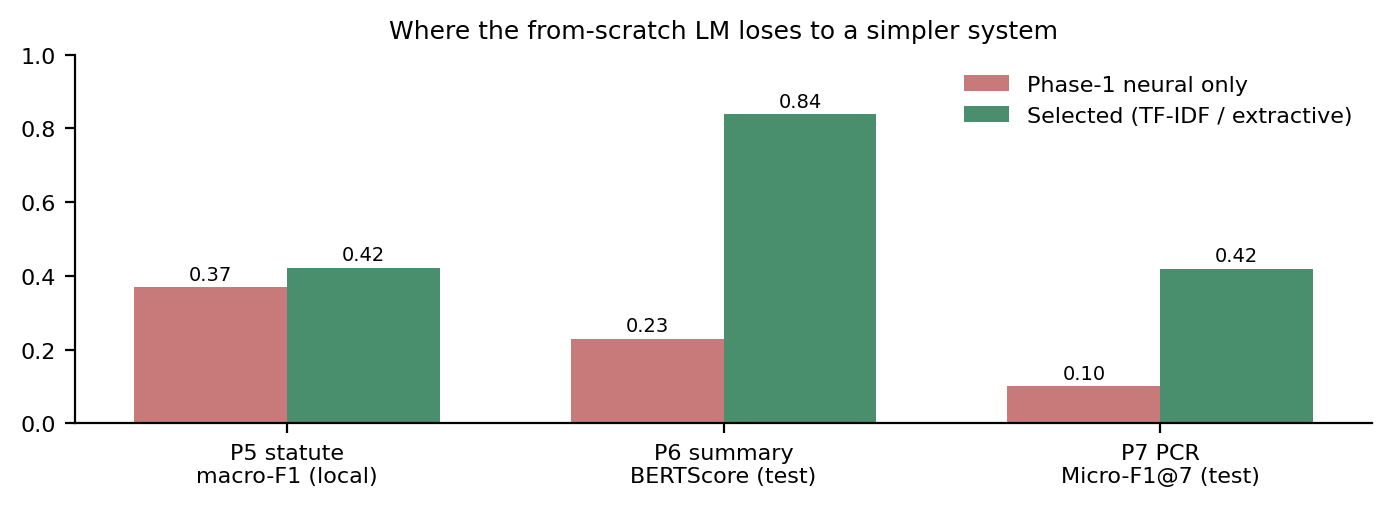
\includegraphics[width=0.88\linewidth]{transfer_gap.png}
\caption{Where a from-scratch 118M LM is a weak matcher on its own. Bars are local or board snapshots of the \emph{neural-only} PEFT path versus the selected TF-IDF/extractive system. Official selected metrics are Table~\ref{tab:leaderboard}.}
\label{fig:gap}
\end{figure}

\section{Error Analysis and Discussion}
\subsection{Phase-wise failure modes}
My Phase~1 model copies the prompt when EOS is late and invents locally fluent citations. Phase~2 misses by a comma or a court suffix; strict span matching treats that as a full miss, so typing quality is understated. Phase~3 confuses Fact with Argument and cannot predict Dissent on documents that simply lack one; PrecedentReliedUpon versus PrecedentOverruled needs more discourse than a mean-pooled sentence. Phase~4 fails on a holding buried in a mid-document double negative, and on ``appeal dismissed'' quoted from a lower court. Phase~5 misses rare IDs and predicts a frequent neighbour of a masked section. My extractive Phase~6 summaries drop a short holding below the word budget; abstractive summaries invent one. Phase~7 leaves relevant cases outside the seven-slot list when they share little surface form with the query (names are masked).

\subsection{What the metrics do not measure}
ROUGE-L and BERTScore reward overlap with a hidden reference, not legal correctness of a holding~\cite{lin2004rouge,zhang2020bertscore}. Strict span-F1 rewards offset perfection. Micro-F1@7 treats a fifth relevant case beyond $K{=}7$ as a miss. If I deployed this stack I would still need a lawyer on the output.

\subsection{Limitations and next experiments}
The 1024-token block and the ban on extra corpora are my ceiling. Under the spec, the next architectural move I would try is a pair scorer that \emph{adds} a feature to TF-IDF rather than replacing the list, and a Phase-6 selector that uses Phase-3 roles as a skeleton. I would not pipeline NER into retrieval until offsets are audited.

\subsection{Surprising findings}
I found that a from-scratch 118M model is a usable token encoder (NER, roles, judgment windows) and a weak semantic matcher on 8k-word name-masked text (Figure~\ref{fig:gap}). That is why my extractive selector beat abstractive continuation, and why I kept a lexical first stage as the PCR serving path even after I trained LoRMA dual-encoders and pair encoders.

\section{Conclusion}
I delivered four in-house legal LMs and seven separately adapted heads. The architectural choices that mattered for me were the efficient GQA body, character-accurate BPE offsets, window packing for long judgments, per-label heads for 100 statutes, extractive length control, and a lexical first stage for retrieval. The choices that did not were a cropped-head encoder, abstractive summarization at this size, and a neural ranker that overwrites TF-IDF. I would keep a compact legal LM under a parameter and data lock as an encoder; it is not, by itself, a retrieval model.

\section*{LLM Usage Declaration}
Completing this section is mandatory. Inconsistent answers relative to the code and the prose will be treated as an integrity issue.
\medskip
\noindent
\textbf{Q1.} Which Large Language Model(s), if any, did you use while completing the competition or writing this report? Give model name and vendor (e.g., none / ChatGPT-4.x / Gemini~x / Claude~x / Grok / Copilot / other). \\[0.6em]
Answer: Free-tier Claude (Anthropic) and free-tier Gemini (Google) for coding assistance and for typesetting this report. No public LLM API was used to train or to score models.
\medskip
\noindent
\textbf{Q2.} For each row, mark Yes or No and state the purpose in one short phrase. ``Yes'' is acceptable only for the uses permitted by the capstone document.
\begin{table}[H]
\centering
\small
\begin{tabular}{>{\raggedright\arraybackslash}p{5.0cm}|c|>{\raggedright\arraybackslash}p{6.6cm}}
\toprule
Part & Used LLM? & Purpose of using the LLM \\
\midrule
Understanding concepts / papers & Yes & Clarify PEFT / CRF / BERTScore definitions \\
Ideation / brainstorming at a high level & Yes & Enumerate legal ablations already suggested by the spec \\
Debugging small ancillary snippets & Yes & Sklearn \texttt{np.matrix} errors, Kaggle unpack, zip schema \\
Plotting / visualization code & Yes & TikZ system diagram in this PDF \\
Grammar / writing style of the report & Yes & Tighten prose against the template checklist \\
Report structure / section wording & Yes & Map experiment logs onto the required sections \\
Designing the model architecture & No & \\
Hyperparameter search / tuning & No & \\
Analysis of results / conclusions & No & \\
Writing the core training / inference code & No & \\
Other (specify) & No & \\
\bottomrule
\end{tabular}
\end{table}
\medskip
\noindent
\textbf{Q3.} Did you refer to sources other than lecture slides and an LLM?
If yes, list them (papers, blogs, GitHub repositories, textbooks, official starter notebook, evaluation scripts). These must also appear in the bibliography when they influenced the method. \\[0.4em]
Answer: Yes. Official CS-781 starter and evaluators; Hugging Face card~\cite{cs781capstone}; papers in the bibliography; sklearn TF-IDF; Kaggle notebook API.
\medskip
\noindent
\textbf{Q4.} Apart from any permitted LLM use, what was \emph{your} contribution? In 8--12 sentences describe your own understanding, architecture decisions, implementation, experiments, and analysis. Name at least two things you tried that failed and what you concluded from them.

I specified the four Phase-1 architectures (causal decoder, windowed hybrid, GQA-efficient, encoder--decoder), the Dice-weighted BPE, and the rule that every later phase must load those weights. I chose LoRMA as the compulsory PEFT method, CRF heads for sequence tasks, window packing for long judgments, and per-label thresholds for 100 statutes. I ran the Codabench loop: local evaluator, zip, upload, and the decision to keep or drop a system. I rejected public legal BERT once the spec forbade it. Two failures that changed the design: a 400-word NER BiLSTM that never saw late entities, which forced character-aligned sliding windows; and dual-encoder / pair-encoder PCR that overwrote a lexical list it could not improve. A third failure, a 12k-word PCR clip, overfit 118 dev queries. Extractive 720-word selection was my decision after abstractive SFT stalled. The conclusions in this report are those architectural outcomes.

\bibliographystyle{ieeetr}
\bibliography{references}
\end{document}
